%\begin{apendicesenv}

\chapter{Protocolo de revisão sistemática sobre técnicas para detecção e reconstrução de olusões parciais em imagens de face}
\label{apen2:RS}

\section{Objetivo}



O objetivo principal dessa revisão sistemática foi realizar um levantamento sistemático do estado de arte, referente a técnicas de detecção e reconstrução de oclusões parciais em imagens de faces humanas visando o reconhecimento biométrico. Mediante esse estudo, foi possível extrair dados para o tema desta dissertação, a fim de conseguir informações pertinentes, como por exemplo: quais algoritmos estão sendo aplicados para detectar oclusões parciais, e reconstruir faces parcialmente ocluídas, quais as métricas de avaliação que são normalmente utilizadas, quais estratégias estão apresentando melhor resultado, quais as condições do ambiente, e quais bases de dados utilizadas.


% ----------------------------------------------
\section{Questões de pesquisa}
Em adição aos objetivos da revisão sistemática elaborada, as questões de pesquisa auxiliam na busca por informações relevantes por meio da leitura integral dos estudos. Tais informações são obtidas após a extração e síntese dos dados extraídos da leitura. As questões de pesquisa levantadas foram:

\begin{enumerate}
\item quais técnicas estão sendo utilizadas para reconstrução de faces humanas e como são aplicadas?	
\item quais as técnicas utilizadas para detecção de oclusões parciais e como são aplicadas?
 \item como os resultados são analisados e comparados?
 \item qual tipo de reconhecimento biométrico foi utilizado?\item Quais bases de dados estão sendo utilizadas?
\end{enumerate}
%---------------------------------------------------

\section{Seleção de fontes}
Para selecionar os estudos primários para essa revisão sistemática, foram utilizadas as três bases indexadoras a seguir:

Os trabalhos devem estar preferencialmente disponíveis na internet, em bases de dados científicas. As seguintes bases foram selecionadas para realização das buscas:

\begin{enumerate}
\item Biblioteca Digital do Scopus (https://www.scopus.com/)
\item Biblioteca Digital do IEEE (http://ieeexplore.ieee.org/Xplore/home.jsp)
\item Biblioteca Digital do Web of Science (https://apps.webofknowledge.com)
\end{enumerate}

A justificativa para a escolha dessas três bases se refere à abrangência, quase total, dos artigos presentes nas bibliotecas digitais com idioma na língua inglesa. Para encontrar tais artigos nas bases indexadoras, foi elaborado uma string de busca para cada uma das bases com os termos descritos mais detalhadamente na seção \ref{ap:palavraschave}. O apêndice \ref{Apen:conducao_Revisao}, apresenta com maiores o processo de seleção de artigos.


%----------------------------------------------------

\section{Palavras-Chave}
\label{ap:palavraschave}
A \textit{String de busca} envolveu as palavras-chave descritas abaixo:

\begin{enumerate}
\item 'occlusion' OR 'occluded';
\item 'detect*' OR 'recogni*' OR 'analys*' OR 'reconstruct*';
\item 'face' OR 'faces' OR 'facial' ;
\item 'biometry*'.
\end{enumerate}

Os artigos retornados pela aplicação da \textit{String} de busca nos motores de busca, foram lidos seus respectivos títulos e resumos.
% -------------------------------------------

\section{Critérios de inclusão}
Para essa revisão sistemática, três critérios de inclusão foram definidos, sendo eles:

I1 - Artigos que abordem métodos e técnicas utilizadas para detecção de oclusão parciais em faces humanas.

I2 - Artigos que abordem técnicas utilizadas para reconstrução de faces humanas.

I3 - Artigos que abordem modelagens híbridas para detecção de oclusões parciais e/ou reconstrução facial. 

%--------------------------------------------

\section{Critérios de exclusão}


E1 - Artigos de revisão serão excluídos.

E2 - Trabalhos que estejam na forma de livros, capítulos de livros, prefácio de eventos, pôster e artigos resumidos.

E3 - Trabalhos que não estejam na língua Inglesa.

E4 - Trabalhos que não sejam revisados por pares.

% -----------------------------------------------

\section{Estratégia de seleção dos dados}

Foi construída uma \textit{String} com palavras-chave e seus sinônimos, onde essa \textit{String} foi submetida nas máquinas de busca. Após a leitura dos resumos e títulos e sua posterior aplicação dos critérios de inclusão e exclusão, com isso os artigos foram selecionados conforme sua adequação juntos aos critérios de inclusão, apresentando relevância daquele artigo perante a pesquisa. 

%------------------------------------------------

\section{Síntese dos dados extraídos}

Após a leitura na íntegra de cada artigo incluído, foi elaborado um formulário de extração dos dados, a fim de serem sintetizados e gerar informações pertinentes, os dados coletados foram:

\begin{enumerate}
\item autores;
\item objetivo do trabalho;
\item estratégia para detecção de oclusão parcial;
\item estratégia para reconstrução de face;
\item base de dados utilizada;
\item forma de avaliação;
\item métricas utilizadas;
\item identificação das vantagens e desvantagens de cada método;
\item resultados obtidos;
\item limitações do trabalho;
\item trabalhos futuros.

\end{enumerate}


\section{Ameaças a validade}


Os resultados da pesquisa podem revelar que as técnicas ou fusões de técnicas apresentadas para detecção de oclusão ou reconstrução de faces não produzem um bom resultado ou não são aplicáveis a tal ambiente de coleta, assim refutando a hipótese de pesquisa. 
Outra possível ameaça que este projeto pode apresentar é a existência de outras técnicas com fins a identificar a parte ocluída em uma imagem facial e/ou reconstruir a face sem finalidades biométricas.


\section{Critérios de qualidade}
Após a seleção dos estudos e a leitura integral de cada um deles, existe a necessidade de realizar uma avaliação subjetiva direcionada ao objetivo da revisão sistemática. Desse modo, alguns critérios de qualidade foram desenvolvidos para tal fim, sendo eles:


Q1 -	Os objetivos da pesquisa são claramente definidos?

Q2 -	O contexto é adequadamente descrito?

Q3 - 	Foram apresentadas técnicas de detecção de oclusões claramente?

Q4 -	Foram apresentadas técnicas de reconstrução facial?

Q5 -	O código de detecção de oclusões foi disponibilizado?

Q6 - 	O código de detecção de reconstrução facial foi disponibilizado?

Q7 -	O ambiente do estudo primário foi apresentado claramente?

Q8 -	A proposta do estudo foi validada?

Q9 -	A proposta é comparada com outro método?

Q10 -	 Foi apresentado o Dataset utilizado?

Q11 - 	 O experimento é aplicado em conjuntos de dados suficientes?

Q12 -	 Os resultados foram apresentados claramente?

Para cada critério de qualidade necessariamente era atribuído uma nota, sendo Sim (S) = 1 ponto, Não (N) = 0 ponto, e Parcialmente (P) = 0,5.



\chapter{Condução da revisão}
\label{apen3:conducao_Revisao}


Após o planejamento da revisão sistemática e definição do protocolo, a condução dos passos consistiram das seguintes etapas: submissão das \textit{strings} nas máquinas de busca do Scopus, IEEE e Web of Science; aplicação dos artigos retornados nas máquinas de busca e aplicação dos critérios de inclusão e exclusão; e extração dos dados dos artigos incluídos e lidos integralmente.

O processo de busca dos artigos foi realizado no período compreendido entre 25 de janeiro e 06 de fevereiro de 2017. A partir dessas buscas 440 artigos foram retornados, de modo que após a aplicação dos critérios de inclusão e exclusão 38 artigos foram selecionados para leitura e análise completa, sendo que após a leitura completa do trabalho foram selecionados 31 artigos com relevante grau de contribuição para a pesquisa. A figura \ref{fig:esquemaconducao} apresenta um esquema do processo de seleção dos artigos.

\begin{figure}[H]
\caption{Processo de seleção dos artigos}
\centering
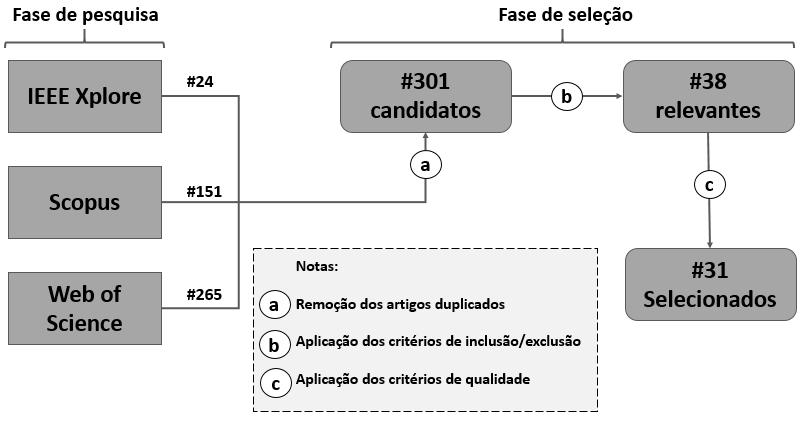
\includegraphics[scale = 0.65]{imgs/conducao.png}
\source{Jonas Mendonça Targino, 2018}
\label{fig:esquemaconducao}
\end{figure}





\chapter{Contextualização da literatura}
\label{apen4:contextualizacao_literatura}


Este  capítulo possui como objetivo principal apresentar um apanhado geral das técnicas para detecção e reconstrução de oclusões parciais em imagens de face visando o reconhecimento biométrico. Essas técnicas foram obtidas graças ao trabalho de \citeonline{Targino2018_wvc} o qual apresentou uma revisão sistemática das técnicas presentes na literatura. 


\section{Escopo dos estudos}

Dentro do conjunto de estudos selecionados e analisados, existem autores que abordam a técnica de detecção de oclusão e paralelamente realizam a reconstrução da face, entretanto em outros trabalhos são implementados apenas uma das duas técnicas. Diante dos trabalhos lidos foi possível perceber que a maioria deles não apresentaram o algoritmo de construção da técnica de forma detalhada. Sendo possível a implementação da técnica mediante a leitura de outros trabalhos com abordagens semelhantes e mais específicas, abrangendo com isso uma maior quantidade de detalhes. É notável perceber que a maioria dos trabalhos abordaram adaptações de técnicas já existentes para detecção e reconstrução de oclusões parciais. 



\section{Bases de dados}
\label{sec:base de dados}

Três bases de dados foram amplamente utilizadas nos trabalhos analisados e esta seção as descreve resumidamente. Em alguns artigos mais de uma base foram utilizadas de modo a possibilitar o uso de uma ou mais bases para o conjunto de treinamento e outra de modo a prover instâncias para o conjunto de teste. Todas as bases de dados utilizadas nos trabalhos abordados na revisão sistemática estão representadas na figura \ref{fig:basesDeDados}, dentre essas apresentadas, aqui será dado maior ênfase nas três bases de dados mais utilizadas, sendo elas:

\begin{itemize}
\item \textbf{AR} esta base de dados foi utilizada em nove dos trabalhos analisados (29\%). Ela possui um pouco mais de 2.600 imagens de face frontal de 100 indivíduos (50 homens e 50 mulheres). De modo que para cada indivíduo são coletadas 26 fotos, estas coletadas sobre duas sessões (dois dias diferentes) separadas e sujeitas a 13 variações de condições, dentre estas estão, diferentes expressões faciais, condições de iluminação e variações de oclusão (com óculos de sol e cachecol). A base de dados encontra-se disponível em \url{http://www2.ece.ohio-state.edu/~aleix/ARdatabase.html};

\item \textbf{YALE B} esta base de dados contém 165 imagens frontais de 10 pessoas, contendo variações de iluminação, expressão e oclusão (baixos níveis de oclusão). A base de dados foi utilizada em quatro dos trabalhos selecionados (14\%), e ela encontra-se disponível em \url{http://www.face-rec.org/databases/};

\item \textbf{FRGC} foi a terceira base de dados mais utilizada, três dos trabalhos analisados (11\%) a utilizaram. Esta base de dados contém 12776 imagens frontais de 222 indivíduos, com 6388 imagens coletadas em ambientes controlados e outras 6388 imagens coletadas na presença de ambientes não controlados. Esta base de dados está disponível em \url{https://www.nist.gov/programs-projects/face-recognition-grand-challenge-frgc}.

\end{itemize}

\begin{figure}[H]
\centering
\caption{Bases de dados utilizadas pelos estudos selecionados}
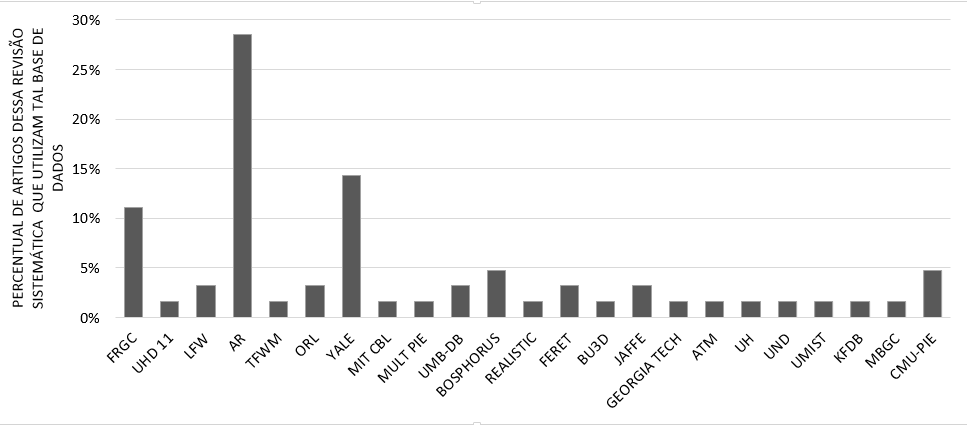
\includegraphics[scale = 0.62]{imgs/bases.png}
\source{Jonas Mendonça Targino, 2018}
\label{fig:basesDeDados}
\end{figure}


Pode-se perceber uma quantidade significativa de bases de dados de face dispostas na literatura, entretanto nem todas as bases disponíveis apresentam uma grande quantidade de imagens bem como também uma grande quantidade de variações existentes. Na tabela \ref{tab:variacoes_bases} são apresentadas algumas das bases mais utilizadas como também número de indivíduos da base, quantidade de imagens, e variações presentes na base. As variações estão apresentadas da forma: (\textbf{i}) representa iluminação; \textit{e} significa expressão; (\textbf{o}) representa oclusão; e \textbf{t} significa variação temporal (ou seja, imagens obtidas da mesma pessoa em diferentes dias).

\begin{table}[H]
	
\centering
\footnotesize
\caption{Bases de dados de domínio público e algumas especificações}
\label{tab:variacoes_bases}

\begin{tabular}{|l|c|c|c|} \hline

\textbf{Bases}& \textbf{Número de indivíduos} & \textbf{Número de imagens} & \textbf{Variações existentes}\\ \hline
      					
AR			&	 100 	& 2600 		& i, e,o, t \\ \hline
Yale B	 	&	15 		& 165 		& i,e\\ \hline
FRGC  		&	222 	& 12776 	& i,e \\ \hline
ORL 		&	40 		& 400 		& p,e\\ \hline
MIT 		&	16 		& 432		& i,p\\ \hline
CMU PIE 	&	68		&41.368 	& p,i,e\\ \hline
FERET		& > 1000 	& > 10000 	& p,i,e,t\\ \hline 
UMIST		& 20		& 564		& p \\ \hline 

		
	\end{tabular}
    
 \source{Jonas Mendonça Targino, 2018}
\end{table}


\section{Técnicas encontradas na literatura}

Após a extração dos dados foi possível analisar as técnicas presentes na literatura para detecção e reconstrução de oclusões parciais com fins biométricos, estas técnicas estão sendo apresentadas com mais detalhes nas subseções \ref{sub:detecção de oclusões} e \ref{sub:reconstrução de faces} logo abaixo.

De modo a gerar uma melhor visualização dos trabalhos selecionados e uma identificação para cada um deles foi elaborada o quadro \ref{tab:autores}, este apresentando a identificação do trabalho, como também o evento em que o mesmo foi publicado.


\begin{quadro}[H]
	\centering
	\caption{Estudos selecionados}
    \resizebox{\columnwidth}{!}{%
		\begin{tabular}{cll} \hline
        %\begin{tabular}{ p{0.2in} p{1.8in}  p{4.7in}   } \hline
		ID	& Autores  & Evento\\ \hline

A1& \cite{[1]bellil2016gappy}  & Multimed Tools Applications\\
A2 & \cite{[2]zhang2016face}  & Chinese Conference on Biometric Recognition\\
A3& \cite{[3]dou2015pose} & Biometrics Theory, Applications and Systems (BTAS)\\
A4 & \cite{[4]wei2014dynamic}  & IEEE Transactions on Information Forensics and Security\\
A5 & \cite{[5]aisha2014face} & KSII Transactions on Internet and Information Systems (TIIS)\\
A6 & \cite{[6]yang2014fast}   & Pattern Recognition\\
%A7 & \cite{[7]venkatakrishnan20143d} & 2014 & periódico & Applied Mechanics \& Materials\\
A7 & \cite{[8]alyuz2014detection}  & International Conference Pattern Recognition (ICPR) \\
A8& \cite{[9]bindu2014inpainting}   & Signal and Image Processing (ICSIP)\\
%A10 & \cite{[10]bindu2013novel} & 2013 & conferência & Advances in Computing, Communications and Informatics (ICACCI)\\
A9 & \cite{[11]lai2013robust}  & International Conference Acoustics, Speech, and Signal Processing (ICASSP)\\
A10  & \cite{[12]sharma2013efficient}& Neurocomputing\\
A11 & \cite{[13]wei2013robust} & International Workshop Biometrics and Forensics (IWBF)\\
A12 & \cite{[14]alyuz20133}  & IEEE Transactions on Information Forensics and Security\\
A13 & \cite{[15]li2013structured}  & IEEE transactions on image processing\\ 
A14 & \cite{[16]min2012inpainting}   & International Conference Image Processing (ICIP)\\
A15 & \cite{[17]alyuz2012robust}  & International Conference Biometrics (ICB)\\
A16 & \cite{[18]zhu2012discriminant} & International Conference Biometrics (ICB)\\
A17 & \cite{[19]song2012three} & IEEE Transactions on Image Processing\\
A18 & \cite{[20]shermina2012recognition}  & International Journal of Pattern Recognition and Artificial Intelligence\\
%A21 & \cite{[21]min2011cap} & 2011 & conferência & Proceedings of the 19th ACM international conference on Multimedia\\
A19 & \cite{[22]chiang2011recognizing}  & International Journal of Innovative Computing, Information and Control\\
A20 & \cite{[23]eum2011face} & Computer Vision and Pattern Recognition Workshops \\
A21 & \cite{[24]passalis2011using}& IEEE Transactions on Pattern Analysis and Machine Intelligence\\
A22 & \cite{[25]deng2011graph}   & IEEE Transactions on Image Processing\\
A23 & \cite{[26]storer2010occlusion}  & Computer Vision and Pattern Recognition Workshops (CVPRW)\\
A24& \cite{[27]yan2010misalignment}& IEEE transactions on image processing\\
A25 & \cite{[28]de2010faro}& IEEE Transactions on Systems, Man, and Cybernetics-Part A: Systems and Humans\\
%A29 & \cite{[29]marcon20093d} & 2009 & conferência & IET\\
%A30 & \cite{[30]du2009analysis} & 2009 & conferência & Information Technology and Applications\\
A26 & \cite{[31]su2009multi}  & International Conference on Biometrics\\
A27 & \cite{[32]wright2009robust}   & IEEE transactions on pattern analysis and machine intelligence\\
%A33 & \cite{[33]heo2007face} & 2007 & conferência & Biometrics Symposium\\
A28 & \cite{[34]zhang2006robust}  & Journal of Multimedia\\
%A35 & \cite{[35]lee2006face} & 2006 & conferência &International Conference Pattern Recognition (ICPR)\\
A29 & \cite{[36]huang2012subface}  & IET biometrics\\
A30 & \cite{[37]hosoi2012restoring} & Computer Vision and Pattern Recognition Workshops (CVPRW)\\
A31 & \cite{[38]tan2005recognizing}  &IEEE Transactions on Neural Networks\\
\hline
		\end{tabular}
        }
        \source{Jonas Mendonça Targino, 2018}
            \label{tab:autores}

\end{quadro}





\subsection{Técnicas para detecção de oclusões parciais}
\label{sub:detecção de oclusões}
Algumas técnicas para detecção de oclusões parciais em imagens de face, coletadas a partir da revisão sistemática estão destacadas no quadro \ref{tab:Tecnicas deteccao}. Após a análise deste quadro podemos enxergar um número considerável de técnicas com tal finalidade.



\nomenclature{IKFDA}{Incremental Kernel Fisher Discriminant Analysis}
\begin{quadro}[H]
	\centering
	\caption{Técnicas para detecção de oclusão}
		\begin{tabular}{p{1.2in} p{4.2in} } \hline

		ID do Artigo  & Nome da Técnica\\ \hline
  
A1& Transformada Wavelet Discreta(DCT) \nomenclature{DCT}{Discrete Wavelet Transform} \\
A2 & Rede Neural Convolucional(CNN) \nomenclature{CNN}{Convolucional Neural NetWork}   \\\
A4,A11& Imagens Dinâmicas para Classes Deformadas(DICW) \nomenclature{DICW}{Dynamic image to class Warping}\\
A5 & Kernel Incremental de Análise Discriminante de Fisher (IKFDA)  \\
A6,A25,A32 & Classificação por Representação Esparsa (SRC)  \nomenclature{SRC}{Sparse Representation  Classification} \\
A14 & Máscara de Projeção FisherFace\\
A7 & Mistura de Modelos Gaussianos (GMM) \nomenclature{GCC}{Gaussian Mixture Models} \\
%A10 & Skin ilumination e SURF\\
A9 & Classificação de regressão linear aparada (TLRC) \nomenclature{TLRC}{trimmed linear regression
classification} \\
A10 & Filtros de Gabor\\
A13 & Estrutura Esparsa de Codificação do Erro(SSEC) \nomenclature{SSEC}{Structured Sparse Error Coding}\\  
A14 & Robusta Análise dos Componentes Principais (RPCA) \nomenclature{RPCA}{Robust Principal Component Analisys} \\
A15 & ICP junto ao modelo genérico facial\\
A16 & Fases de Gabor com SLRDA\\
A18 &  Bloco de Algoritmo de correspondência (BMA) \nomenclature{BMA}{Block Matching Algorithm}\\
%A21 & Skin color com DTW\\
A19 & Descoberta Iterativa de Faces(IFR) \nomenclature{IFR}{Iterative Face Recovery}\\
A20& Manipulação de Oclusões Excepcionais(EOH) \nomenclature{EOH}{Exceptional Occlusion Handling}\\
%A21 & UR3DS\\
A23 & Técnica do Espaço de Cores (CST) \nomenclature{CST}{Color Space Technique}\\
A24 & Desalinhamento Robusto (MAR)\\
A25 & Reconhecimento Facial contra Oclusão(FARO)\nomenclature{FARO}{Face Recognition Against Occlusion}\\
%A30 & Skin color\\
A26 & Multi Visões de Alinhamento de Faces \\
A28 & Memória de Kernel Associativo(KAM) \nomenclature{KAM}{Kernel Associative Memory}\\
A29 & Modelos Ocultos Markovianos (HMM) \nomenclature{HMM}{Hidden Markov Models}\\
A31 & Mapa de Auto Organização(SOM) \nomenclature{SOM}{Self Organizaton Maps}\\

 \hline
		
		\end{tabular}
		\source{Jonas Mendonça Targino, 2018}
	\label{tab:Tecnicas deteccao}
\end{quadro}

	


\subsection{Técnicas para reconstrução de imagens de Faces}
\label{sub:reconstrução de faces}

Após a fase de detecção da oclusão na imagem da face, torna-se imprescindível a reconstrução da oclusão, de modo a possibilitar a identificação biométrica. A partir da leitura dos artigos foi possível extrair algumas técnicas para reconstrução de faces. As técnicas encontradas são apresentadas no quadro \ref{tab:Tecnicas reconstrução}. Analisando este quadro pode-se perceber um pequeno número de técnicas com tal finalidade quando comparado com as técnicas para detecção de oclusão. 


\begin{quadro}[H]
	\centering
	\caption{Técnicas para reconstrução de faces}
		\begin{tabular}{p{1.1in} p{4.4in} } \hline

		ID do Artigo & Nome da Técnica\\ \hline
  
A1 & Rede Neural de Onda de Multi-Biblioteca (MLWNN) \nomenclature{MLWNN}{Multi Library Wavelet Neural Network} \\
%A3 & 3DAFM\\
A4,A27 & SRC\\
A7 & Inpainting for big data (IBD) \nomenclature{IBD}{Inpainting for Big Data}\\
A9 & TLRC\\
A10 & Eigenfaces com Eigenfaces reformados de Gabor(RGEF)\nomenclature{RGEF}{Reformed Gabor Eigen Faces} \\
A12,A15 & Gappy Análise dos Componentes Principais (GPCA) \nomenclature{GPCA}{Gappy Principal Component Analysis} \\
A16 & Fases de Gabor com RSLDA\\
%A17 & CRBF netwok \\ é aplicada apenas para 3D
A18,A19,A24 & Eigenfaces \nomenclature{PCA}{Principal Component Analysis} \\
A22 & Grafos Laplacianos\\
A23 & CST + Modelos de Formas Ativas (ASM) \nomenclature{ASM}{Active Shape Model} e PCA\\
A28 & KAM \\
A30 & Pesos Rápidos de Análises de Componentes Principais (FWPCA) \nomenclature{FWPCA}{Fast-Weighted Principal Component Analysis}\\
                
 \hline
		\end{tabular}
		\source{Jonas Mendonça Targino, 2018}
	\label{tab:Tecnicas reconstrução}
\end{quadro}



\section{Considerações finais do apêndice}

Considerando a importância das técnicas de detecção e reconstrução de oclusões parciais em imagens de face visando o reconhecimento biométrico. Neste apêndice foi apresentada uma revisão sistemática de literatura a respeito das técnicas presentes no estado da arte com fins de detecção e/ou reconstrução de oclusões parciais em imagens de de face.

Com a análise dos artigos incluídos percebeu-se que existe uma quantidade considerável de técnicas presentes na literatura, entretanto essas técnicas apresentam configurações de execuções limitadas, não seguindo um rigor sistemático de bases de dados utilizadas, como também disponibilidade de códigos ou pseudo-códigos para futuras replicações por outras pessoas interessadas na área.

Foi possível concluir com essa revisão sistemática, que a área apresenta uma certa instabilidade em relação a padrões de execuções, tipos de oclusões, sem contar que alguns autores não utilizam um estudo comparativo mais aprofundado com outras técnicas presentes no estado da arte. Como também grande parte dos artigos não apresentam fins que possibilitem replicação do trabalho pela comunidade científica.


\chapter{Matrizes de confusão}
\label{apen6:matrizes_confusao}
Abaixo são apresentadas as matrizes de confusão de cada técnica, de modo que após a análise da diagonal é possível perceber qual classe teve um maior índice de acertos, como também seus falsos positivos e falsos negativos.

\section{Técnicas baseadas em subespaço}

\begin{figure}[H]
\caption{Matriz de confusão da técnica Asymmetrical PCA na base de dados AR}
\centering
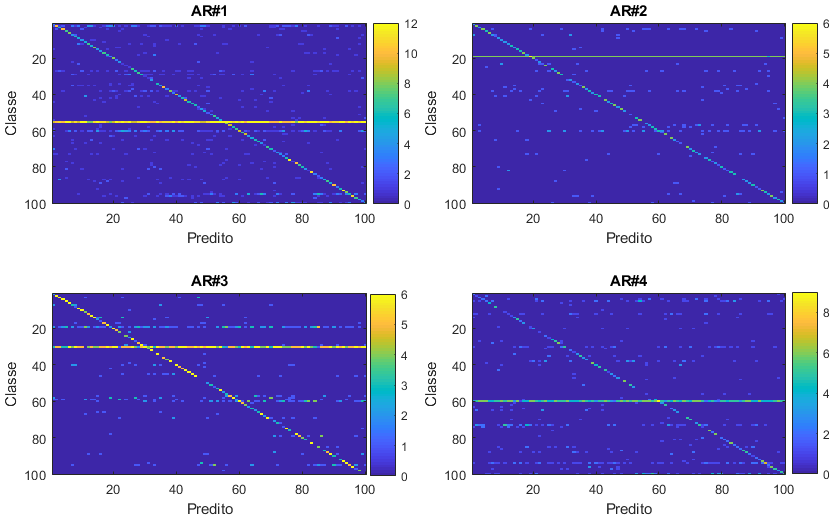
\includegraphics[scale = 0.65]{imgs4/matrizes_confusao/APCA}
\source{Jonas Mendonça Targino, 2018}
\end{figure}

\begin{figure}[H]
\caption{Matriz de confusão da técnica Fast Recursive PCA na base de dados AR}
\centering
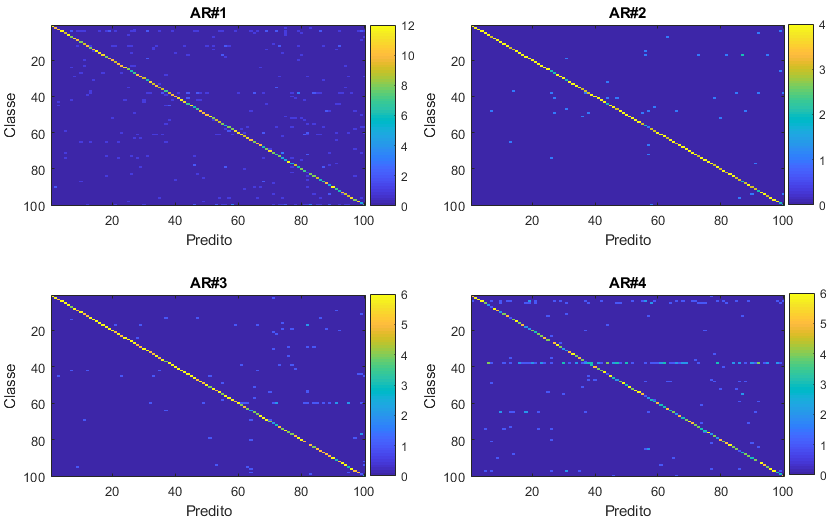
\includegraphics[scale = 0.65]{imgs4/matrizes_confusao/FastRecPCA}
\source{Jonas Mendonça Targino, 2018}
\end{figure}

\begin{figure}[H]
\caption{Matriz de confusão da técnica Fisherfaces na base de dados AR}
\centering
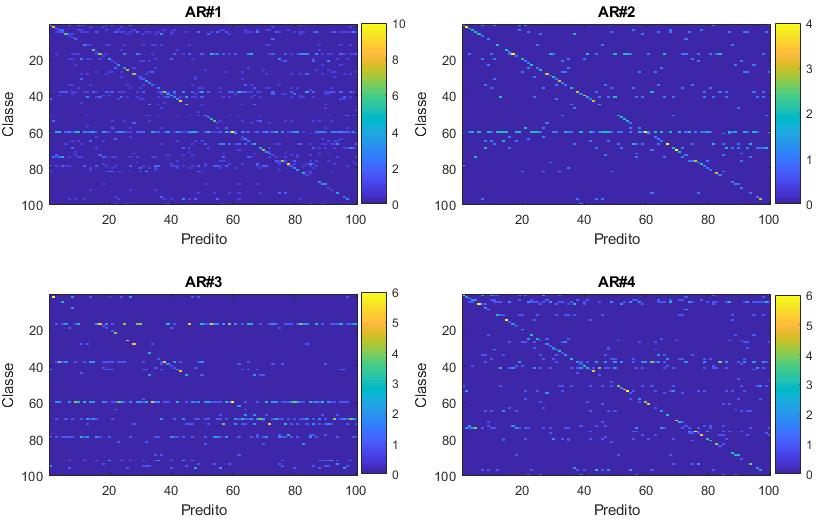
\includegraphics[scale = 0.65]{imgs4/matrizes_confusao/fisherfaces}
\source{Jonas Mendonça Targino, 2018}
\end{figure}


\begin{figure}[H]
\caption{Matriz de confusão da técnica Fast Robust PCA na base de dados AR}
\centering
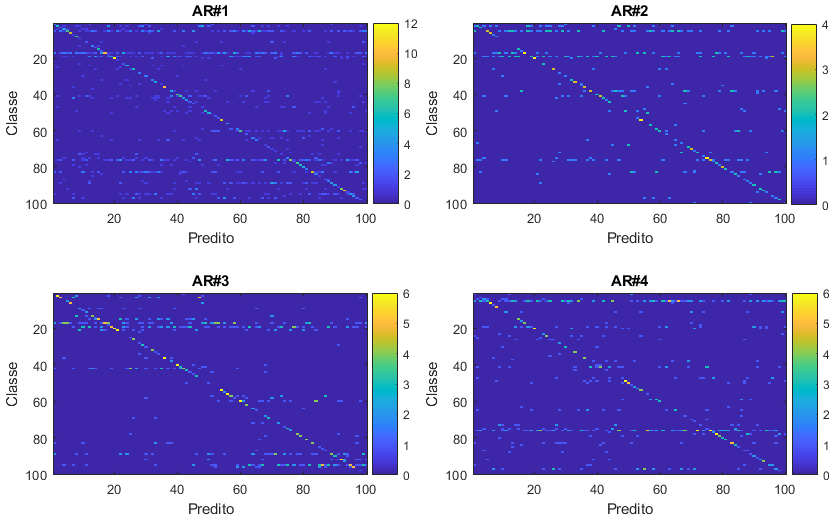
\includegraphics[scale = 0.65]{imgs4/matrizes_confusao/FRPCA}
\source{Jonas Mendonça Targino, 2018}
\end{figure}

\begin{figure}[H]
\caption{Matriz de confusão da técnica Gappy PCA na base de dados AR}
\centering
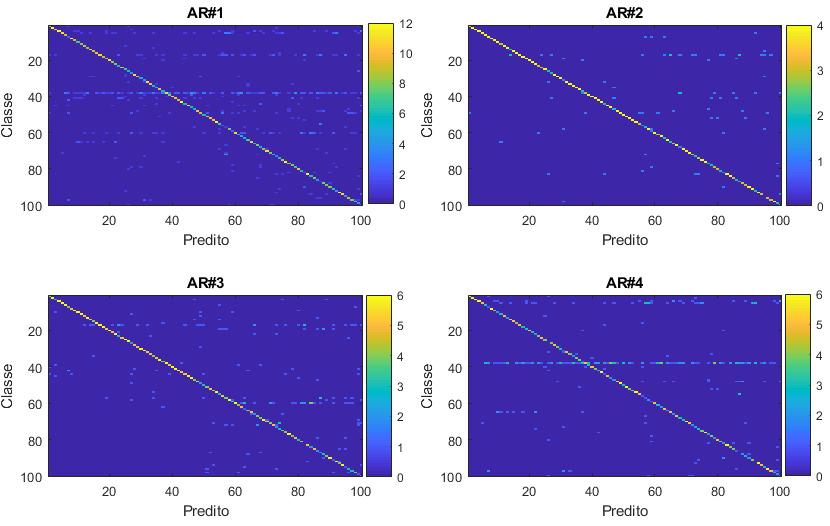
\includegraphics[scale = 0.65]{imgs4/matrizes_confusao/GPCA}
\source{Jonas Mendonça Targino, 2018}
\end{figure}

\begin{figure}[H]
\caption{Matriz de confusão da técnica PCA na base de dados AR}
\centering
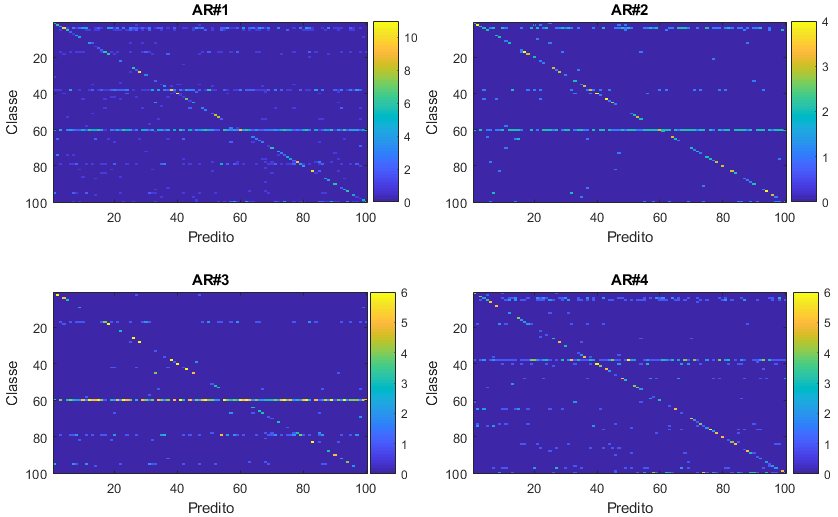
\includegraphics[scale = 0.65]{imgs4/matrizes_confusao/PCA}
\source{Jonas Mendonça Targino, 2018}
\end{figure}


\begin{figure}[H]
\caption{Matriz de confusão da técnica Recursive PCA na base de dados AR}
\centering
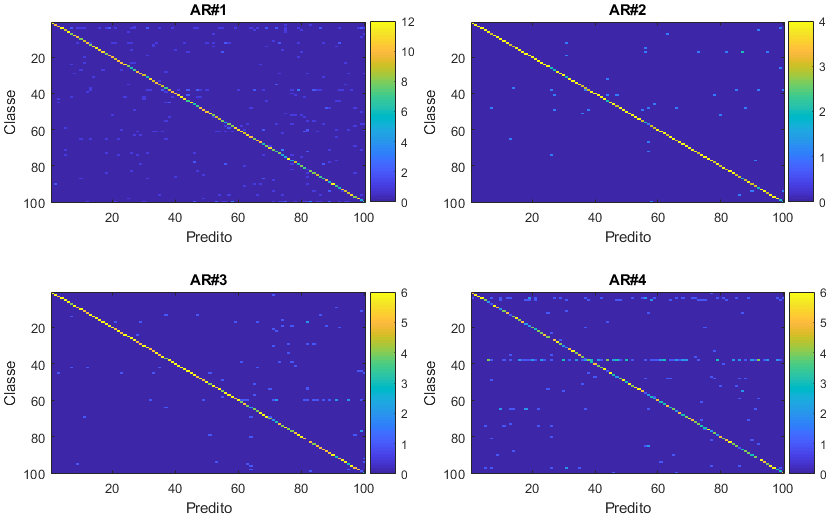
\includegraphics[scale = 0.65]{imgs4/matrizes_confusao/RecPCA}
\source{Jonas Mendonça Targino, 2018}
\end{figure}


\begin{figure}[H]
\caption{Matriz de confusão da técnica SRC com Fast Recursive PCA na base de dados AR}
\centering
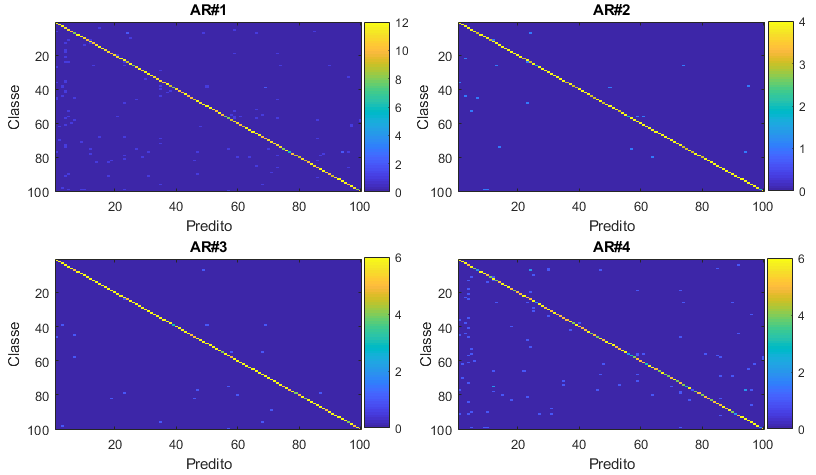
\includegraphics[scale = 0.65]{imgs4/matrizes_confusao/src_fast_rec_PCA}
\source{Jonas Mendonça Targino, 2018}
\end{figure}




%%%%%%%%%%%%%%%%%%%%%%%%%%%%%%%%%%%%%%%%%%%%%%%%%%%
%%%%%%%%%%%%%%%%%%%%%%%%%%%%%%%%%%%%%%%%%%%%%%%%%%%
\section{Técnicas baseadas em modelo}



\begin{figure}[H]
\caption{Matriz de confusão da técnica SRC com grafo de Poisson na base de dados AR}
\centering
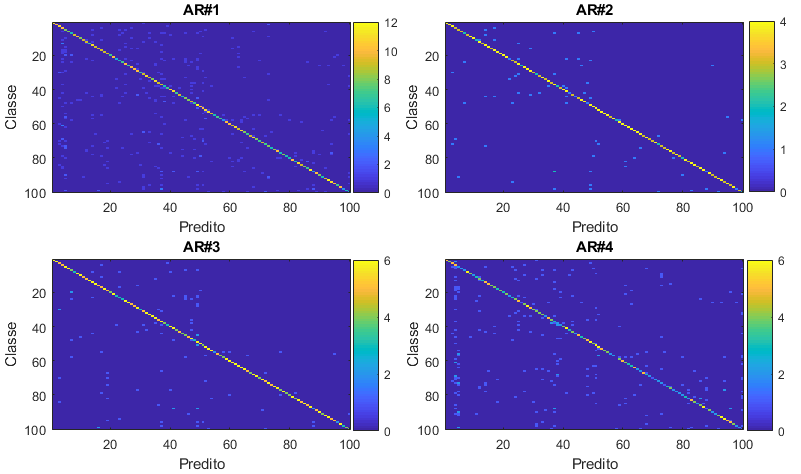
\includegraphics[scale = 0.65]{imgs4/matrizes_confusao/SRC_GP}
\source{Jonas Mendonça Targino, 2018}
\end{figure}



\begin{figure}[H]
\caption{Matriz de confusão da técnica SRC com grafo Laplaciano na base de dados AR}
\centering
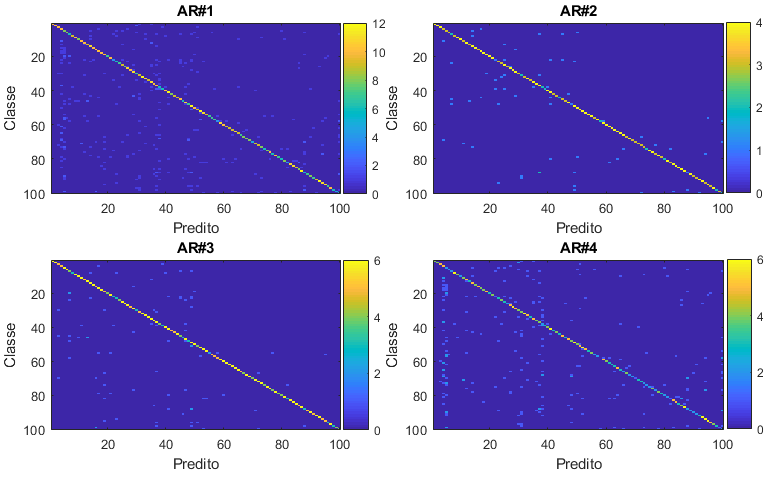
\includegraphics[scale = 0.65]{imgs4/matrizes_confusao/SRC_GL}
\source{Jonas Mendonça Targino, 2018}
\end{figure}


\begin{figure}[H]
\caption{Matriz de confusão da técnica SSIMGL na base de dados AR}
\centering
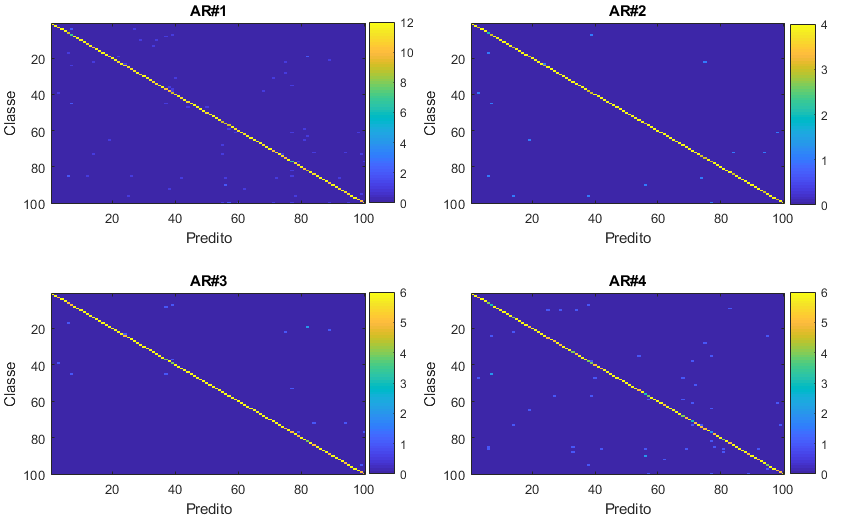
\includegraphics[scale = 0.65]{imgs4/matrizes_confusao/ssimgl}
\source{Jonas Mendonça Targino, 2018}
\end{figure}

%\end{apendicesenv}




